\documentclass[aspectratio=43]{beamer}

%\documentclass[handout]{beamer}
%% To make 4 per page
%\usepackage{pgfpages}
%\mode<handout>{\setbeamercolor{background canvas}{bg=white}}
%\pgfpagesuselayout{4 on 1}[letterpaper,landscape]%,border shrink=5mm]

\usetheme{default}
\usepackage{bm}
\usepackage{colortbl}

\usepackage{amsmath,amssymb,amsthm}
%\usepackage{subfigure}


% Fields and the like
\def\IC{\mathbb{C}}
\def\IF{\mathbb{F}}
\def\II{\mathbb{I}}
\def\IM{\mathbb{M}}
\def\IN{\mathbb{N}}
\def\IP{\mathbb{P}}
\def\IR{\mathbb{R}}
\def\IZ{\mathbb{Z}}

% Bold lowercase
\def\ba{\mathbf{a}}
\def\bb{\mathbf{b}}
\def\bc{\mathbf{c}}
\def\bd{\mathbf{d}}
\def\be{\mathbf{e}}
\def\bf{\mathbf{f}}
\def\bh{\mathbf{h}}
\def\bi{\mathbf{i}}
\def\bj{\mathbf{j}}
\def\bk{\mathbf{k}}
\def\bn{\mathbf{n}}
\def\bp{\mathbf{p}}
\def\br{\mathbf{r}}
\def\bs{\mathbf{s}}
\def\bu{\mathbf{u}}
\def\bv{\mathbf{v}}
\def\bw{\mathbf{w}}
\def\bx{\mathbf{x}}
\def\by{\mathbf{y}}
\def\bz{\mathbf{z}}

% Bold capitals
\def\bB{\mathbf{B}}
\def\bD{\mathbf{D}}
\def\bF{\mathbf{F}}
\def\bG{\mathbf{G}}
\def\bI{\mathbf{I}}
\def\bL{\mathbf{L}}
\def\bN{\mathbf{N}}
\def\bR{\mathbf{R}}
\def\bS{\mathbf{S}}
\def\bT{\mathbf{T}}
\def\bX{\mathbf{X}}

% Bold numbers
\def\b0{\mathbf{0}}

% Bold greek
\bmdefine{\bmu}{\bm{\mu}}
\def\bphi{\bm{\phi}}
\def\bvarphi{\bm{\varphi}}

% Bold red sentence
\def\boldred#1{{\color{red}\textbf{#1}}}
\def\defword#1{{\color{orange}\textbf{#1}}}

% Caligraphic letters
\def\A{\mathcal{A}}
\def\B{\mathcal{B}}
\def\C{\mathcal{C}}
\def\D{\mathcal{D}}
\def\E{\mathcal{E}}
\def\F{\mathcal{F}}
\def\G{\mathcal{G}}
\def\I{\mathcal{I}}
\def\L{\mathcal{L}}
\def\M{\mathcal{M}}
\def\P{\mathcal{P}}
\def\R{\mathcal{R}}
\def\S{\mathcal{S}}
\def\T{\mathcal{T}}
\def\U{\mathcal{U}}
\def\V{\mathcal{V}}

% tt font for code
\def\code#1{{\tt #1}}

% Operators and special symbols
\def\nbOne{{\mathchoice {\rm 1\mskip-4mu l} {\rm 1\mskip-4mu l}
{\rm 1\mskip-4.5mu l} {\rm 1\mskip-5mu l}}}
\def\cov{\ensuremath{\mathsf{cov}}}
\def\Var{\ensuremath{\mathsf{Var}\ }}
\def\Im{\textrm{Im}\;}
\def\Re{\textrm{Re}\;}
\def\det{\ensuremath{\mathsf{det}}}
\def\diag{\ensuremath{\mathsf{diag}}}
\def\nullspace{\ensuremath{\mathsf{null}}}
\def\nullity{\ensuremath{\mathsf{nullity}}}
\def\rank{\ensuremath{\mathsf{rank}}}
\def\range{\ensuremath{\mathsf{range}}}
\def\sgn{\ensuremath{\mathsf{sgn}}}
\def\Span{\ensuremath{\mathsf{span}}}
\def\tr{\ensuremath{\mathsf{tr}}}
\def\imply{$\Rightarrow$}
\def\restrictTo#1#2{\left.#1\right|_{#2}}
\newcommand{\parallelsum}{\mathbin{\!/\mkern-5mu/\!}}

% The beamer bullet (in base colour)
\def\bbullet{\leavevmode\usebeamertemplate{itemize item}\ }

% Theorems and the like
\newtheorem{proposition}[theorem]{Proposition}
\newtheorem{property}[theorem]{Property}
\newtheorem{importantproperty}[theorem]{Property}
\newtheorem{importanttheorem}[theorem]{Theorem}
%\newtheorem{lemma}[theorem]{Lemma}
%
%\usecolortheme{orchid}
\setbeamertemplate{theorems}[numbered]
%\usecolortheme{orchid}
%\setbeamertemplate{theorems}[ams style]
%\setbeamertemplate{theorems}[numbered]

%% Listings
\usepackage{listings}
\definecolor{mygreen}{rgb}{0,0.6,0}
\definecolor{mygray}{rgb}{0.5,0.5,0.5}
\definecolor{mymauve}{rgb}{0.58,0,0.82}
\definecolor{mygold}{rgb}{1,0.843,0}
\definecolor{myblue}{rgb}{0.537,0.812,0.941}

\definecolor{lgreen}{rgb}{0.6,0.9,.6}
\definecolor{lred}{rgb}{1,0.5,.5}

\lstloadlanguages{R}
\lstset{ %
  language=R,
  backgroundcolor=\color{black!95},   % choose the background color
  basicstyle=\footnotesize\ttfamily,        % size of fonts used for the code
  breaklines=true,                 % automatic line breaking only at whitespace
  captionpos=b,                    % sets the caption-position to bottom
  commentstyle=\color{mygreen},    % comment style
  escapeinside={\%*}{*)},          % if you want to add LaTeX within your code
  keywordstyle=\color{myblue},       % keyword style
  stringstyle=\color{mygold},     % string literal style
  keepspaces=true,
  columns=fullflexible,
  tabsize=4,
}
% Could also do (in lstset)
% basicstyle==\fontfamily{pcr}\footnotesize


% Get rid of navigation stuff
\setbeamertemplate{navigation symbols}{}

% Set footline/header line
\setbeamertemplate{footline}
{%
\quad p. \insertpagenumber \quad--\quad \insertsection\vskip2pt
}
% \setbeamertemplate{headline}
% {%
% \quad\insertsection\hfill p. \insertpagenumber\quad\mbox{}\vskip2pt
% }


\makeatletter
\newlength\beamerleftmargin
\setlength\beamerleftmargin{\Gm@lmargin}
\makeatother

%%%%%%% 
%% Definitions in yellow boxes
\usepackage{etoolbox}
\setbeamercolor{block title}{use=structure,fg=structure.fg,bg=structure.fg!05!bg}
\setbeamercolor{block body}{parent=normal text,use=block title,bg=block title.bg!20!bg}

\BeforeBeginEnvironment{definition}{%
	\setbeamercolor{block title}{fg=black,bg=yellow!20!white}
	\setbeamercolor{block body}{fg=black, bg=yellow!05!white}
}
\AfterEndEnvironment{definition}{
	\setbeamercolor{block title}{use=structure,fg=structure.fg,bg=structure.fg!20!bg}
	\setbeamercolor{block body}{parent=normal text,use=block title,bg=block title.bg!50!bg, fg=black}
}
\BeforeBeginEnvironment{importanttheorem}{%
	\setbeamercolor{block title}{fg=black,bg=red!20!white}
	\setbeamercolor{block body}{fg=black, bg=red!05!white}
}
\AfterEndEnvironment{importanttheorem}{
	\setbeamercolor{block title}{use=structure,fg=structure.fg,bg=structure.fg!20!bg}
	\setbeamercolor{block body}{parent=normal text,use=block title,bg=block title.bg!50!bg, fg=black}
}
\BeforeBeginEnvironment{theorem}{%
	\setbeamercolor{block title}{fg=white,bg=red!30!black}
	\setbeamercolor{block body}{fg=white, bg=red!10!black}
}
\AfterEndEnvironment{theorem}{
	\setbeamercolor{block title}{use=structure,fg=structure.fg,bg=structure.fg!20!bg}
	\setbeamercolor{block body}{parent=normal text,use=block title,bg=block title.bg!50!bg, fg=black}
}
\BeforeBeginEnvironment{importantproperty}{%
	\setbeamercolor{block title}{fg=black,bg=red!50!white}
	\setbeamercolor{block body}{fg=black, bg=red!30!white}
}
\AfterEndEnvironment{importantproperty}{
	\setbeamercolor{block title}{use=structure,fg=structure.fg,bg=structure.fg!20!bg}
	\setbeamercolor{block body}{parent=normal text,use=block title,bg=block title.bg!50!bg, fg=black}
}


%%%%%%%%%%%%%%%%%
\usepackage{tikz}
\usetikzlibrary{shapes,arrows}
\usetikzlibrary{positioning}
\usetikzlibrary{shapes.symbols,shapes.callouts,patterns}
\usetikzlibrary{calc,fit}
\usetikzlibrary{backgrounds}
\usetikzlibrary{decorations.pathmorphing,fit,petri}
\usetikzlibrary{automata}
\usetikzlibrary{fadings}
\usetikzlibrary{patterns,hobby}

\usepackage{pgfplots}
\pgfplotsset{compat=1.6}
\pgfplotsset{ticks=none}

\usetikzlibrary{decorations.markings}
\usetikzlibrary{arrows.meta}
\tikzset{>=stealth}

\tikzstyle{cloud} = [draw, 
ellipse,
fill=red!20, 
node distance=0.87cm,
minimum height=2em]
\tikzstyle{line} = [draw, 
-latex', 
color=yellow]


% Beginning of a section
% \AtBeginSection[]{
% 	{
% 		\setbeamercolor{background canvas}{bg=orange!10}
% 		\begin{frame}[noframenumbering,plain]
% 			\framesubtitle{\nameofthepart Chapter \insertromanpartnumber \ -- \iteminsert{\insertpart}}
% 			\tableofcontents[currentsection,currentsubsection]
% 		\end{frame}
% 	\addtocounter{page}{-1}
% 	%\addtocounter{framenumber}{-1} 
% 	}
% }


%%% SLIDES COLOURING

%\usecolortheme{owl}

\setbeamerfont{frametitle}{series=\bfseries}
\setbeamercolor{frametitle}{fg=black!05,bg=black}

\setbeamerfont{framesubtitle}{size=\normalfont\tiny}
\setbeamercolor{framesubtitle}{fg=black!05}

\setbeamercolor{background canvas}{bg=black}
\setbeamercolor{normal text}{fg=black!10}



\definecolor{bottomcolour}{rgb}{0.32,0.3,0.38}
\definecolor{middlecolour}{rgb}{0.08,0.08,0.16}
\definecolor{mycolor}{rgb}{0.4,0.4, 0.4}
% Beginning of a section
\AtBeginSection[]{
	{
		%\setbeamercolor{background canvas}[vertical shading][top=bottomcolour, middle=middlecolour, bottom=black]
		\setbeamertemplate{background canvas}[vertical shading][bottom=bottomcolour,top=black!20]
    % \setbeamertemplate{background canvas}{
    %   \begin{tikzpicture}%[remember picture,overlay]
    %     \shade[top color=yellow!75!green!33,
    %     bottom color=blue!66!green!33,
    %     middle color=blue!6!green!33]
    %   \end{tikzpicture}
    % }
    \begin{frame}[noframenumbering,plain]
			\framesubtitle{\nameofthepart Chapter \insertromanpartnumber \ -- \iteminsert{\insertpart}}
			\tableofcontents[currentsection,currentsubsection]
		\end{frame}
	\addtocounter{page}{-1}
	}
}
% Beginning of a section
\AtBeginSubsection[]{
	{
		%\setbeamercolor{background canvas}[vertical shading][top=bottomcolour, middle=middlecolour, bottom=black]
		%\setbeamertemplate{background canvas}[vertical shading][bottom=bottomcolour,top=black!20]
    \setbeamertemplate{background canvas}{
      \begin{tikzpicture}%[remember picture,overlay]
        \shade[top color=yellow!75!green!33,
        bottom color=blue!66!green!33,
        middle color=blue!6!green!33]
      \end{tikzpicture}
    }
    \begin{frame}[noframenumbering,plain]
			\framesubtitle{\nameofthepart Chapter \insertromanpartnumber \ -- \iteminsert{\insertpart}}
			\tableofcontents[currentsection,currentsubsection]
		\end{frame}
	\addtocounter{page}{-1}
	}
}

% Colours for special pages
\def\extraContent{yellow!20}

%% Allow to change slide colour
%% From: https://tex.stackexchange.com/questions/8043/change-the-background-color-of-a-frame-in-beamer
\defbeamertemplate*{background canvas}{mydefault}{%
  \ifbeamercolorempty[bg]{background canvas}{}{\color{bg}\vrule width\paperwidth height\paperheight}% copied beamer default here
}
\defbeamertemplate*{background canvas}{bg}{%
  \color{lightgray!20}\vrule width\paperwidth height\paperheight% added bg color
}
\BeforeBeginEnvironment{frame}{%
  \setbeamertemplate{background canvas}[mydefault]%
}
\makeatletter
\define@key{beamerframe}{bg}[true]{%
  \setbeamertemplate{background canvas}[bg]%
}
\makeatother
% Use with
%\begin{frame}
% \frametitle{Normal}
%\end{frame} 
%\begin{frame}[bg]
% \frametitle{With bg}
%\end{frame}


%% Vertical alignment on pages
%% From: https://tex.stackexchange.com/questions/148365/how-do-i-ask-beamer-to-exactly-fill-up-a-slide
%% Turn on with
%% \stretchon
%% (outside slide), and off with
%% \stretchoff
% \def\itemsymbol{$\blacktriangleright$}
% \let\svpar\par
% \let\svitemize\itemize
% \let\svenditemize\enditemize
% \let\svitem\item
% \let\svcenter\center
% \let\svendcenter\endcenter
% \let\svcolumn\column
% \let\svendcolumn\endcolumn
% \def\newitem{\renewcommand\item[1][\itemsymbol]{\vfill\svitem[##1]}}%
% \def\newpar{\def\par{\svpar\vfill}}%
% \newcommand\stretchon{%
%   \newpar%
%   \renewcommand\item[1][\itemsymbol]{\svitem[##1]\newitem}%
%   \renewenvironment{itemize}%
%     {\svitemize}{\svenditemize\newpar\par}%
%   \renewenvironment{center}%
%     {\svcenter\newpar}{\svendcenter\newpar}%
%   \renewenvironment{column}[2]%
%     {\svcolumn{##1}\setlength{\parskip}{\columnskip}##2}%
%     {\svendcolumn\vspace{\columnskip}}%
% }
% \newcommand\stretchoff{%
%   \let\par\svpar%
%   \let\item\svitem%
%   \let\itemize\svitemize%
%   \let\enditemize\svenditemize%
%   \let\center\svcenter%
%   \let\endcenter\svendcenter%
%   \let\column\svcolumn%
%   \let\endcolumn\svendcolumn%
% }
% \newlength\columnskip
% \columnskip 0pt



\title{Introduction to mathematical modelling of avian influenza in livestock}
\author{Julien Arino}
\date{April 2023}


\begin{document}
%\stretchon

% The title page
\begin{frame}[noframenumbering,plain]
  \titlepage
\end{frame}
\addtocounter{page}{-1}

% The title page
\begin{frame}[noframenumbering,plain]
  \tableofcontents[hidesubsections]
\end{frame}
\addtocounter{page}{-1}


%%%%%%%%%%%%%%%%%%%
%%%%%%%%%%%%%%%%%%%
%%%%%%%%%%%%%%%%%%%
%%%%%%%%%%%%%%%%%%%
\section{AI characteristics}

%%%%%%%%%%%%%%%%%%%
%%%%%%%%%%%%%%%%%%%
\subsection{Overview}

\begin{frame}{Avian influenza}
  \begin{minipage}{0.4\textwidth}
    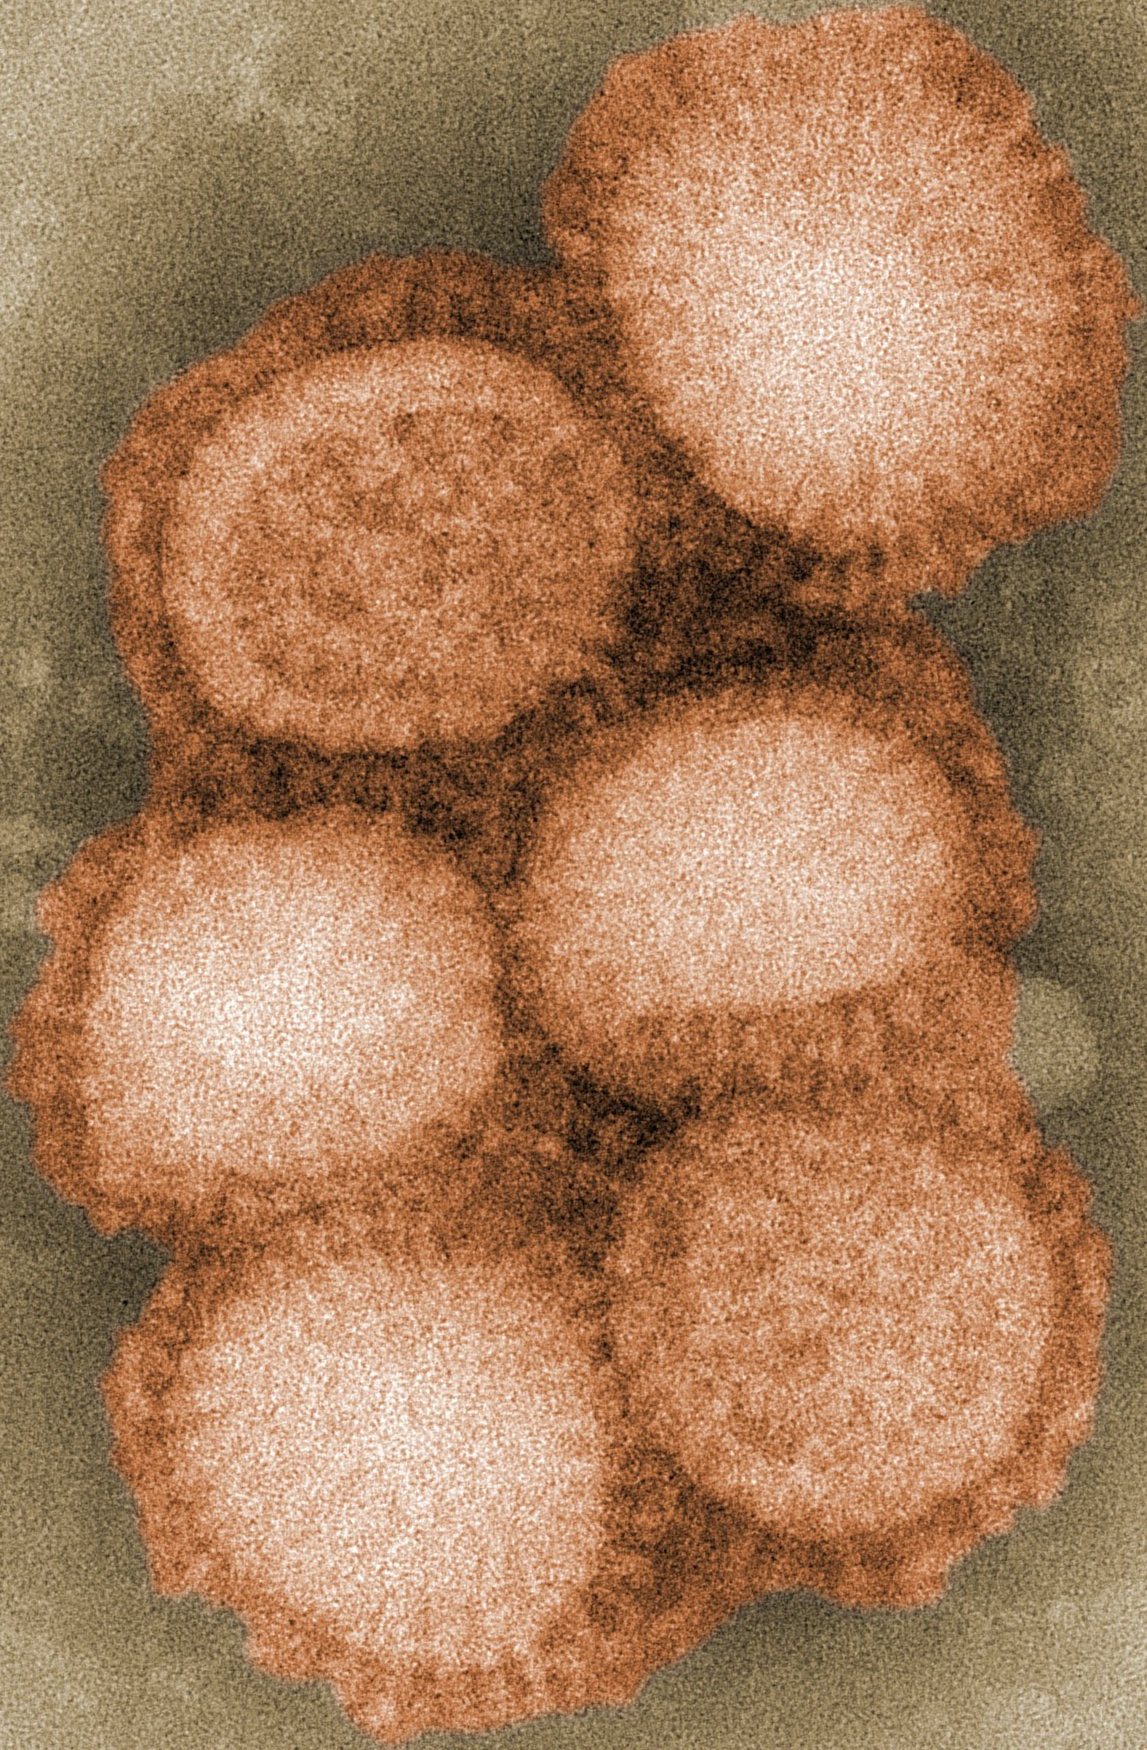
\includegraphics[width=1.1\textwidth]{../FIGS/H1N1_navbox}
  \end{minipage}
  \begin{minipage}{0.55\textwidth}
    \begin{itemize}
      \item Caused by Influenza A virus
      \vskip1cm
      \item Adapted to birds but can also stably adapt and sustain P2P transmission
    \end{itemize}
  \end{minipage}
\end{frame}

\begin{frame}{High pathogenicity avian influenza (HPAI)}
  \begin{itemize}
    \item HPAI A virus subtype H5N1: emerging avian influenza virus causing global concern as a potential pandemic threat
    \vfill
    \item H5N1 has killed millions of poultry throughout Asia, Europe, and Africa
    \vfill
    \item Coexistence of human flu viruses and avian flu viruses (especially H5N1) will provide an opportunity for genetic material to be exchanged between species-specific viruses, possibly creating a new virulent influenza strain that is easily transmissible and lethal to humans
    \vfill
    \item CFR for humans with H5N1 is 60\%
  \end{itemize}
\end{frame}

\begin{frame}
  Global concern because it involves multiple bird species, both wild and livestock
\end{frame}

\subsection{History of AI outbreaks}
% \maxFrameImageBottomTitle{../FIGS/AI-cases-animals1}{test}
% \maxFrameImage{../FIGS/AI-cases-animals2}
% \maxFrameImage{../FIGS//AI-cases-animals3}
% \maxFrameImage{../FIGS/AI-cases-humans}




%%%%%%%%%%%%%%%%%%%
\maxFrameImageBottomTitle{../FIGS/Alexander-history-AI-outbreaks-inverted}{Alexander/Vaccine 25 (2007)}

%%%%%%%%%%%%%%%%%%%
\maxFrameImage{../FIGS/LupianiReddy-AI-history-cover-inverted}
\maxFrameImage{../FIGS/LupianiReddy-AI-history-events-inverted}
\maxFrameImage{../FIGS/LupianiReddy-AI-history-events2-inverted}
\maxFrameImage{../FIGS/LupianiReddy-AI-history-events3-inverted}


%%%%%%%%%%%%%%%%%%%
%%%%%%%%%%%%%%%%%%%
\subsection{Mechanisms of spread}

%%%%%%%%%%%%%%%%%%%
\maxFrameImage{../FIGS/Sonnberg_etal-HPAI-natural-history-cover-inverted.png}
\maxFrameImage{../FIGS/Sonnberg_etal-HPAI-natural-history-interactions-inverted.png}
\maxFrameImage{../FIGS/Sonnberg_etal-HPAI-natural-history-periods-inverted.png}
\maxFrameImage{../FIGS/Sonnberg_etal-HPAI-natural-history-history-inverted.png}

%%%%%%%%%%%%%%%%%%%
%%%%%%%%%%%%%%%%%%%
\subsection{Where does one find the virus?}
\maxFrameImage{../FIGS/Beato_etal-AI-poultry-products-cover-inverted}
\maxFrameImage{../FIGS/Beato_etal-AI-poultry-products-HPAI-inverted}
\maxFrameImage{../FIGS/Beato_etal-AI-poultry-products-LPAI-inverted}



%%%%%%%%%%%%%%%%%%%
%%%%%%%%%%%%%%%%%%%
%%%%%%%%%%%%%%%%%%%
%%%%%%%%%%%%%%%%%%%
\section{Modelling AI}

\begin{frame}{Mathematical modelling of AI}
  A lot more popular than FMD!
  \vfill
  There are \emph{many} mathematical models
  \vfill
  However, most models look at zoonotic aspects, i.e., include a human component
\end{frame}

%%%%%%%%%%%%%%%%%%%
\subsection{A review of Stegeman \emph{et al}}
\maxFrameImage{../FIGS/Stegeman_etal-control-HPAI-models-cover-inverted}
\maxFrameImage{../FIGS/Stegeman_etal-control-HPAI-models-analytical-vs-simulation-inverted}
\maxFrameImage{../FIGS/Stegeman_etal-control-HPAI-models-transmission1-inverted}
\maxFrameImage{../FIGS/Stegeman_etal-control-HPAI-models-transmission2-inverted}

%%%%%%%%%%%%%%%%%%%
\subsection{A within-host model of Xie \emph{et al}}
\maxFrameImage{../FIGS/Xie_etal-H9N2-within-host-cover-inverted}
\maxFrameImage{../FIGS/Xie_etal-H9N2-within-host-model-inverted}
\maxFrameImage{../FIGS/Xie_etal-H9N2-within-host-different-models-AIC-inverted}

%%%%%%%%%%%%%%%%%%%
\subsection{A within-host model of Hagenaars \emph{et al}}
\maxFrameImage{../FIGS/Hagenaars_etal-immune-response-AI-cover-inverted}
\maxFrameImage{../FIGS/Hagenaars_etal-immune-response-AI-flow-inverted}


%%%%%%%%%%%%%%%%%%%
\subsection{A model of Liu \emph{et al}}
\maxFrameImage{../FIGS/Liu_etal-H5N1-cover-inverted}
%\maxFrameImage{../FIGS/Liu_etal-H5N1-model-inverted}

\begin{frame}{3 types of birds $+$ environment}
  \begin{itemize}
    \item Poultry (mainly chicken), $c$
    \item Wild birds who die after H5N1 infection, $w$
    \item Wild birds who survive after H5N1 infection, $d$
    \item $V$ virus density in the environment
  \end{itemize}
\end{frame}

\begin{frame}
  \begin{center}
    \def\vertskip{*-2}
    \def\horzskip{*2.5}
    \begin{tikzpicture}[scale=1, transform shape]
      \node [rectangle, fill=gray!10, text=black] at (0\horzskip,-1\vertskip) (Sc) {$S_c$};
      \node [rectangle, fill=gray!10, text=black] at (1\horzskip,-1\vertskip) (Ic) {$I_c$};
      \node [rectangle, fill=gray!10, text=black] at (0\horzskip,0\vertskip) (Sw) {$S_w$};
      \node [rectangle, fill=gray!10, text=black] at (1\horzskip,0\vertskip) (Ew) {$E_w$};
      \node [rectangle, fill=gray!10, text=black] at (2\horzskip,0\vertskip) (Iw) {$I_w$};
      \node [rectangle, fill=gray!10, text=black] at (0\horzskip,1\vertskip) (Sd) {$S_d$};
      \node [rectangle, fill=gray!10, text=black] at (1\horzskip,1\vertskip) (Id) {$I_d$};
      \node [rectangle, fill=gray!10, text=black] at (2\horzskip,1\vertskip) (Rd) {$R_d$};
      \node [rectangle, fill=gray!10, text=black] at (3\horzskip,0\vertskip) (V) {$V$};
      %% Flows between compartments
      \path [line, very thick] (Sc.north east) to node [midway, above] (TextNode) {$\alpha_c$} (Ic.north west);
      \path [line, very thick, bend left] (Ic) to node [midway, above, sloped] (TextNode) {$r_c$} (V);
      \path [line, very thick, sloped] (Sw.north east) to node [midway, above] (TextNode) {$\alpha_{ew},\alpha_{iw}$} (Ew.north west);
      \path [line, very thick] (Ew) to node [midway, above] (TextNode) {$\mu_w$} (Iw);
      \path [line, very thick, bend left=45] (Ew) to node [midway, above, sloped] (TextNode) {$r_{ew}$} (V);
      \path [line, very thick] (Iw) to node [midway, above] (TextNode) {$r_{iw}$} (V);
      \path [line, very thick] (Sd.north east) to node [midway, above] (TextNode) {$\alpha_d$} (Id.north west);
      \path [line, very thick] (Id) to node [near end, above] (TextNode) {$\gamma_d$} (Rd);
      \path [line, very thick] (Id) to node [midway, above, sloped] (TextNode) {$r_d$} (V);
      \path [line, very thick, bend left=45] (Rd) to node [midway, below] (TextNode) {$\eta_d$} (Sd);
      %% Flows into compartments
      \path [line, very thick, dashed] (0.5\horzskip,-0.85\vertskip) to node [midway, below] (TextNode) {$\beta_{c}$} (Ic.south west);
      \path [line, very thick, dashed] (0.5\horzskip,0.15\vertskip) to node [midway, below] (TextNode) {$\beta_{w}$} (Ew.south west);
      \path [line, very thick, dashed] (0.5\horzskip,1.15\vertskip) to node [midway, below] (TextNode) {$\beta_{d}$} (Id.south west);
      %% Flows out of compartments
      \path [line, very thick] (Ic) to node [midway, right] (TextNode) {$d_{ic}$} ++(0\horzskip,-0.5\vertskip);
      \path [line, very thick] (Iw) to node [midway, right] (TextNode) {$d_{iw}$} ++(0\horzskip,-0.5\vertskip);
      \path [line, very thick] (V.north east) to node [midway, above] (TextNode) {$\delta$} ++(0.5\horzskip,0\vertskip);
      \path [line, very thick] (V.south east) to node [midway, below] (TextNode) {$d_v$} ++(0.5\horzskip,0\vertskip);
    \end{tikzpicture}    
  \end{center}  
\end{frame}



%%%%%%%%%%%%%%%%%%%
\maxFrameImage{../FIGS/MaWang-AI-seasonal-cover-inverted}

\begin{frame}{Divide year in two periods}
  \begin{itemize}
    \item During the \emph{reproductive period}, denoted $p$, poultry can reproduce
    \vfill
    \item During the \emph{overwintering period}, denoted $w$, poultry does not reproduce and AI emerges. Further subdivided
    \begin{itemize}
      \item infection phase
      \item disease-control phase
    \end{itemize}
  \end{itemize}
  \vfill
  Individuals infected with AI do not recover
\end{frame}

\begin{frame}
  \begin{align*}
  S_{n+1}^p &= f_r(N_n^w)(S_n^w+vI_n^w)+u_pS_n^w \\
  I_{n+1}^p &= u_p\sigma_pI_n^w \\
  S_{n+1} &= S_{n+1}^p\Phi\left(
    \beta\frac{I_{n}1^p}{N_{n+1}^p}
  \right) \\
  I_{n+1} &= S_{n+1}^p\left(1-\Phi\left(
    \beta\frac{I_{n}1^p}{N_{n+1}^p}
  \right)\right)+I_{n+1}^p \\
  S_{n+1}^w &= u_wS_{n+1} \\
  I_{n+1}^w &= u_w\sigma_wI_{n+1}
  \end{align*}
  where
  \begin{align*}
    N_n^p &= S_n^p+I_n^p \\
    N_n^w &= S_n^w+I_n^w \\
    N_n &= S_n+I_n 
  \end{align*}
\end{frame}

\begin{frame}{Assumptions on $\Phi$}
  $\Phi$ satisfies
  \begin{itemize}
    \item $\Phi:[0,\infty)\to[0,1]$
    \item $\Phi(0)=1$, $\lim_{x\to\infty}\Phi(x)=0$
    \item $\Phi'(x)<0$ and $\Phi''(x)\geq 0$ for all $x\in[0,\infty)$
    \item $-\Phi'(x)x<1$ for all $x\in[0,\infty)$
  \end{itemize}
\end{frame}

\begin{frame}
  They then conduct a thorough analysis of the system using 
  \[
    \R^\star = \frac{au_w}{1-u_pu_w}
  \]
  and
  \[
    \R_0=\frac{-\beta u_wu_p\sigma_p\sigma_w\Phi'(0)}{1-u_p\sigma_pu_w\sigma_w}
  \]
  \vfill
  \begin{proposition}
    Let $\R^\star>1$. If $\R_0<1$, DFE is GAS; if $\R_0>1$, DFE is unstable and system is uniformly persistent
  \end{proposition}
  Additional results (flip bifurcation, Hopf bifurcation, etc.) based on another $\hat\R_0$
\end{frame}

%%%%%%%%%%%%%%%%%%%
%\maxFrameImage{../FIGS/deJonmgHagenaars-cover-inverted}


%%%%%%%%%%%%%%%%%%%
\maxFrameImage{../FIGS/Barnes_etal-cover-inverted}

\begin{frame}{A branching process model}
  $X$ r.v. ``number of newly infected birds in a generation''
  \vfill
  Generation time: average time in days between successive generations in infection process
  \vfill
  Assume Poisson branching process for transmission, mean transmission rate $\lambda=p_L^BL+p_G^BM$
  \vfill
  Local contact probability $p_L^B$ between birds within social group of size $L$ and smaller global component between all birds within the flock of size $M$ with lower infectious contact probability $p_G^B$
\end{frame}

\begin{frame}
  Then probability generating function for number of newly infected birds in each generation is
  \[
    \Phi_X(s)=\exp\left(
      (p_L^BL+p_G^BM)(s-1)
    \right)
  \]
  and probability of extinction $q$ the smallest root in $(0,1]$ of
  \[
    q=\Phi_X(q)
  \]
  \vfill
  Reproduction number is
  \[
    R_\star = p_L^BL+p_G^BM
  \]
\end{frame}

\begin{frame}
  They then derive a model for infection within a cage
  \vfill
  And models for emergence of HPAI from LPAI
  \vfill
  Then look at various population structures (barn and free-range layer flocks, caged layer flocks, barn and free-range meat flocks, LPAI introductions)
\end{frame}

\maxFrameImage{../FIGS/Barnes_etal-enterprise-characteristics-inverted}
\maxFrameImage{../FIGS/Barnes_etal-proba-outbreak-inverted}


%%%%%%%%%%%%%%%%%%%
\maxFrameImage{../FIGS/Tiensin_etal-H5N1-Thailand-cover-inverted}
\maxFrameImage{../FIGS/Tiensin_etal-H5N1-Thailand-model-inverted}
\maxFrameImage{../FIGS/Tiensin_etal-H5N1-Thailand-characteristics-inverted}
\maxFrameImage{../FIGS/Tiensin_etal-H5N1-Thailand-estimates-inverted}
%%%%%%%%%%%%%%%%%%%
\maxFrameImage{../FIGS/Nickbakhsh_etal-cocirculation-LPAI-HPAI-cover-inverted}
\maxFrameImage{../FIGS/Nickbakhsh_etal-cocirculation-LPAI-HPAI-hypotheses-inverted}
\maxFrameImage{../FIGS/Nickbakhsh_etal-cocirculation-LPAI-HPAI-flow-inverted}
%\maxFrameImage{../FIGS/Nickbakhsh_etal-cocirculation-LPAI-HPAI-model1-inverted}
%\maxFrameImage{../FIGS/Nickbakhsh_etal-cocirculation-LPAI-HPAI-model2-inverted}



\end{document}
